\documentclass{article}
\usepackage{longtable}
\usepackage{makecell}
\usepackage{float}
\usepackage{graphicx}
\usepackage{bm}
\usepackage{amsmath}
\usepackage{placeins}
\usepackage{threeparttable} 
\usepackage{multirow}
\usepackage{aligned-overset}
\usepackage[slantfont,boldfont]{xeCJK}
\usepackage{fontspec}
\counterwithin{figure}{section}
\renewcommand{\arraystretch}{1.5}
\setCJKmainfont{SimSun}
\setmainfont{SimSun}
\setsansfont{SimSun}

\title{衍射光栅特性研究报告}
\author{2411545 邱凯锐}
\date{2025.3.31}

\begin{document}
\maketitle
\section{实验目的}
\begin{itemize}
    \item (1)了解分光仪的结构
    \item (2)掌握分光仪的调节和使用方法
    \item (3)了解光栅的分光特性
    \item (4)测量光栅常数
    \item (5)测量汞光谱中两条黄线的波长并计算角色散
\end{itemize}
\section{实验原理}
\subsection{分光仪}
\begin{figure}[h]
    \centering
    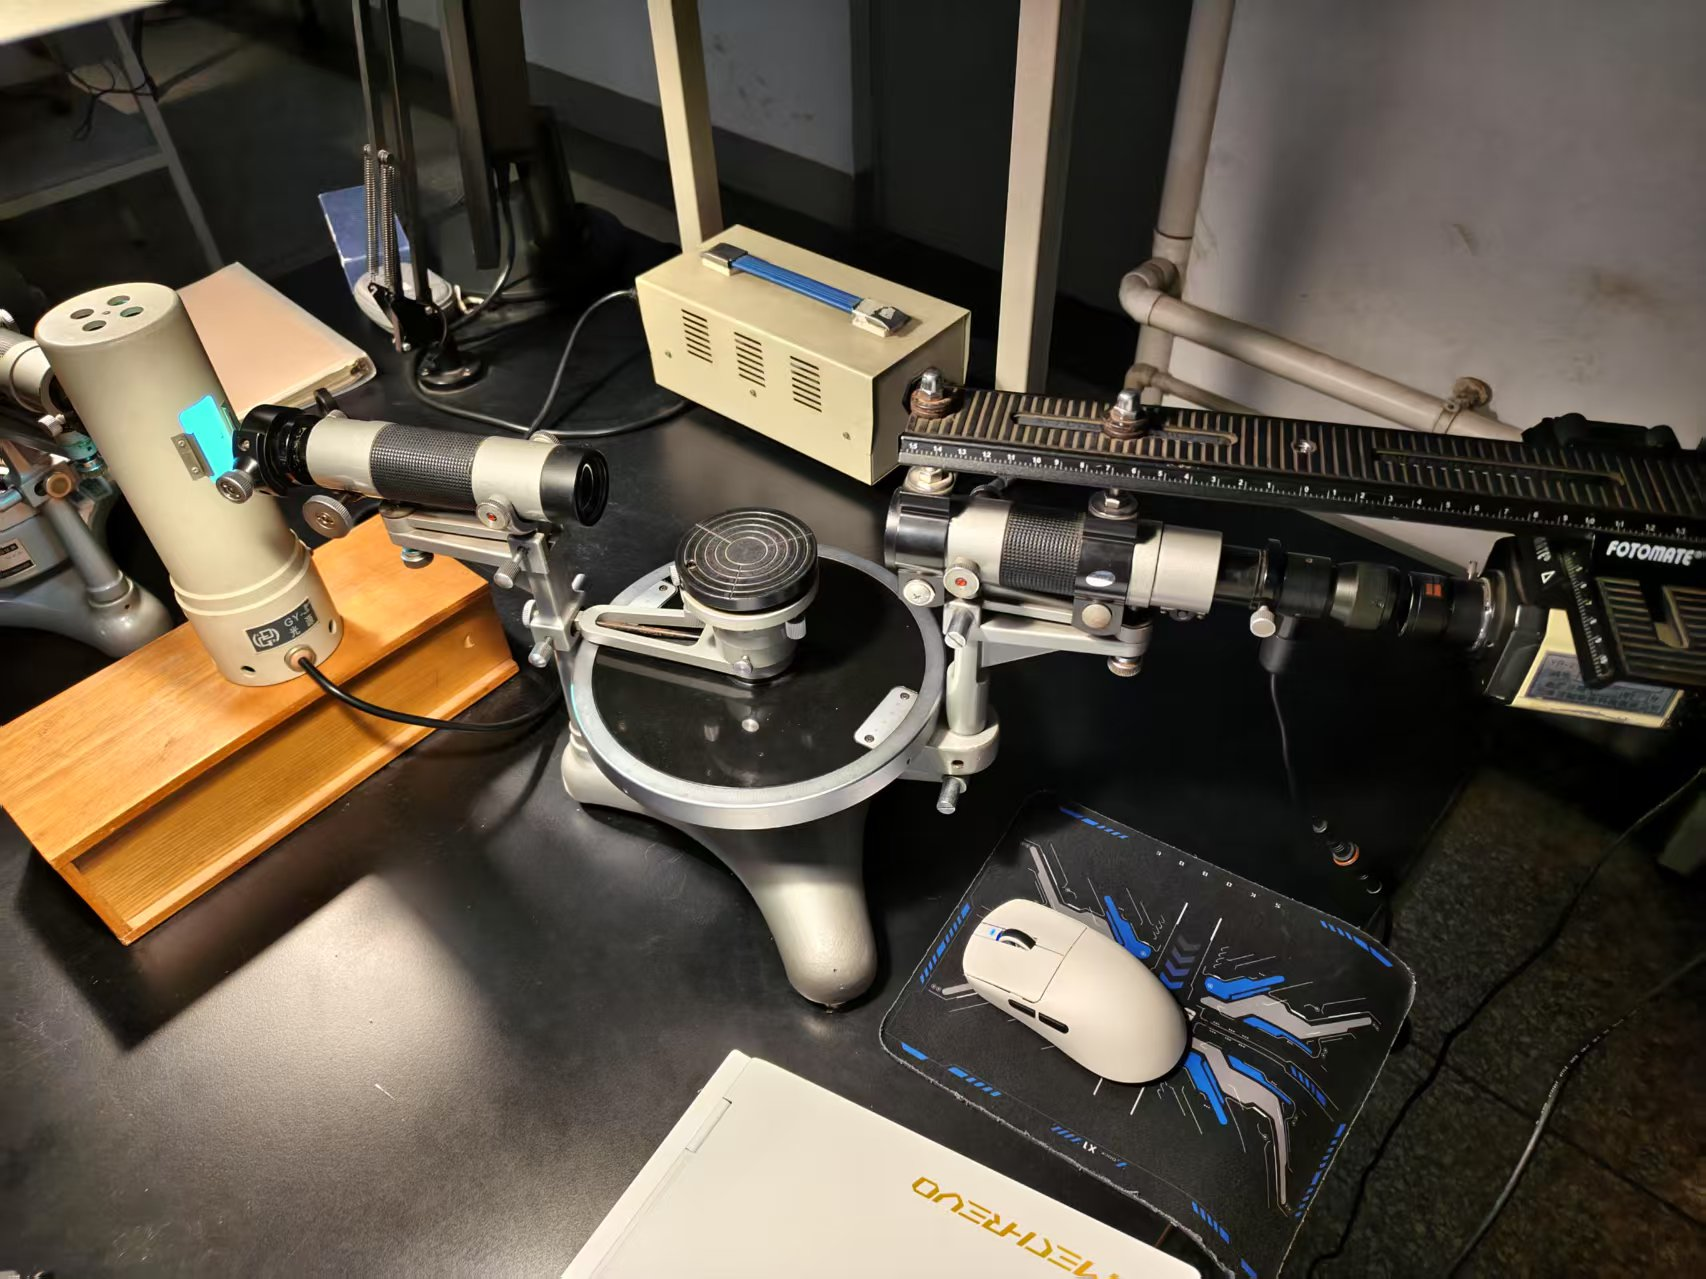
\includegraphics[width=6cm]{3.1.jpg}
    \caption{分光仪}
\end{figure}
分光仪一般由底座、望远镜、平行光管、载物台和读数装置组成。其中读数装置由游标盘和刻度盘组成。由于游标盘和刻度盘中心不在同一点上,会产生偏心差,所以设置两个游标盘,取测量值的平均值$\alpha =\frac{\beta_1+\beta_2}{2}$,以消除偏心差。
\subsection{光栅原理}
\hspace*{2em}二元光栅是平行等宽、等间距的多狭缝,它的分光原理如Figure 2.1所示。狭缝\(S\)处于透镜\(L_{1}\)的焦平面上,并认为它是无限细的;\(G\)是衍射光栅,它有\(N\)个宽度为\(a\)的狭缝,相邻狭缝间不透明部分的宽度为\(b\)。如果自透镜\(L_{1}\)出射的平行光垂直照射在光栅上,透镜\(L_{2}\)将与光栅法线成\(\theta\)角的光会聚在焦平面上的\(P\)点。
光栅在\(\theta\)方向上有干涉主极大的条件为:
\begin{equation}
(a + b)\sin\theta = k\lambda
\end{equation}
是垂直入射条件下的光栅方程。式中,\(k\)为光谱的级次、\(\lambda\)是波长、\(\theta\)是衍射角、\(a+b\)是光栅常数,通常用\(d\)表示,\(d = a + b\)。
\begin{figure}[h]
    \centering
    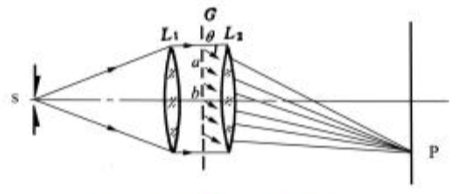
\includegraphics[width=6cm]{2.1.png} % 请将此处文件名替换为实际图片文件名
    \caption{光栅的分光原理}
\end{figure}
\section{实验装置}
\begin{itemize}
    \item 分光仪
    \item 平面透射光栅
    \item 半透半反镜
    \item 低压汞灯
\end{itemize}
\begin{figure}[ht]
    \centering
    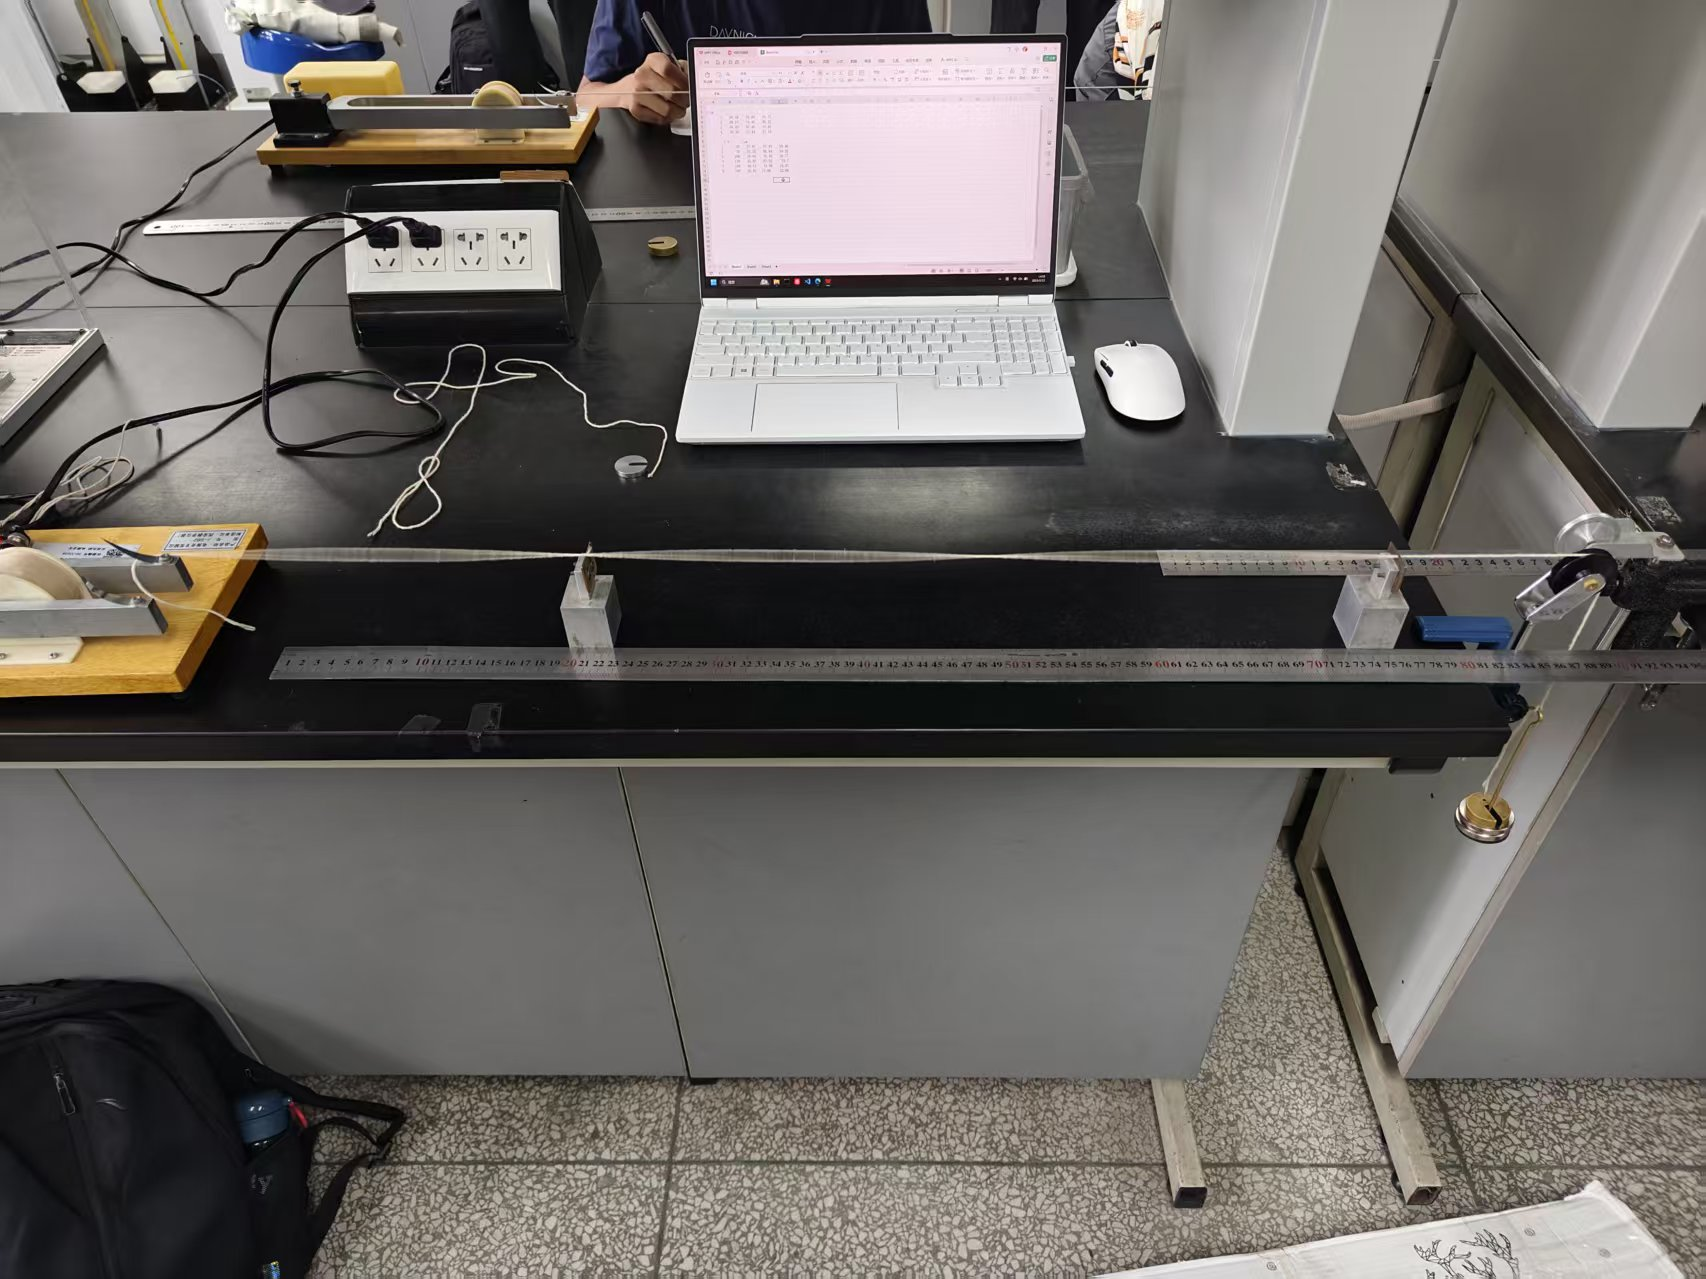
\includegraphics[width=6cm]{3.jpg}
    \caption{实验装置}
\end{figure}
\section{实验内容}
1. \textbf{调节分光仪}\\
\hspace*{2em}利用半透半反镜和各半调节法将望远镜光轴和载物台转轴调节至垂直。\\
2. \textbf{调节光栅}\\
\hspace*{2em}由于在实验中将用垂直入射的光栅方程作为测量公式,因此放置在载物台上的光栅必须满足下列条件:
\begin{itemize}
    \item (1)平行光垂直照射在光栅表面。
    \item (2)光栅的刻痕垂直于刻度盘平面,即与仪器转轴平行。
    \item (3)狭缝与光栅刻痕平行。
\end{itemize}
在步骤1的基础上,再次使用各半调节法并且调节平行光管,使装置满足上述条件。\\
3.\textbf{利用汞绿线测定光栅常数}\\
\hspace*{2em}测量汞光谱中绿线\(\lambda = 546.1nm\) 的\(\pm1\)、\(\pm2\) 级光谱之间的夹角,\(2\theta_{1}\) 和 \(2\theta_{2}\),利用式\((1)\),分别求出两个光栅常数,并取它们的平均值作为测量结果。\\
4.\textbf{测定汞光谱中两条黄线的波长,并计算角色散$\frac{\Delta \theta}{\Delta \lambda}=\frac{k}{d\cos \theta}$}
\section{实验数据}
\begin{figure}[h]
    \centering
    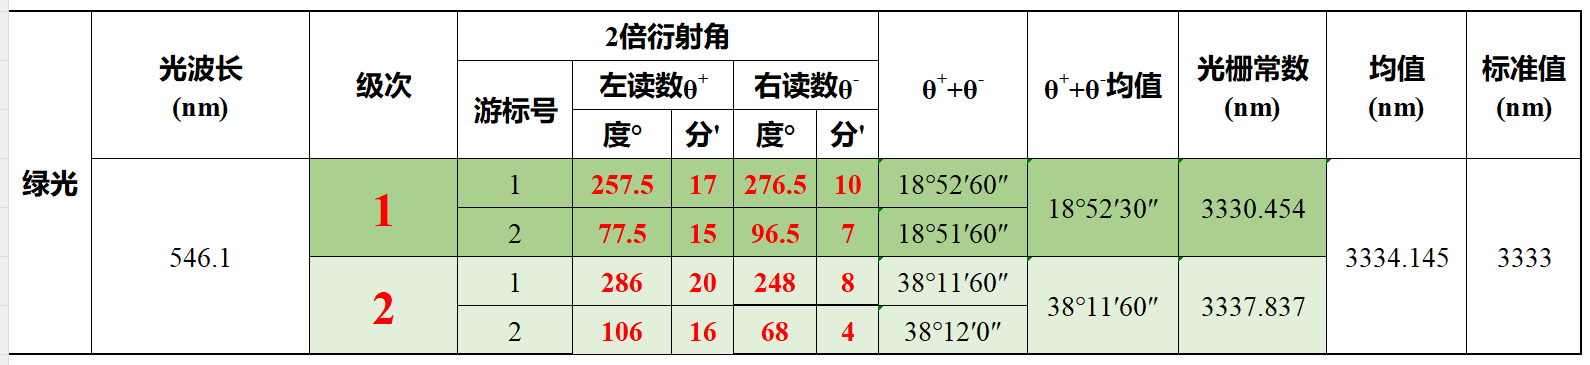
\includegraphics[width=12cm]{data1.png}
    \caption{测量光栅常数实验数据}
\end{figure}
相对误差$E=\frac{d_{测量}-d_{理论}}{d_{理论}}\approx 3.43\times 10^{-4} $\\
\begin{figure}[h]
    \centering
    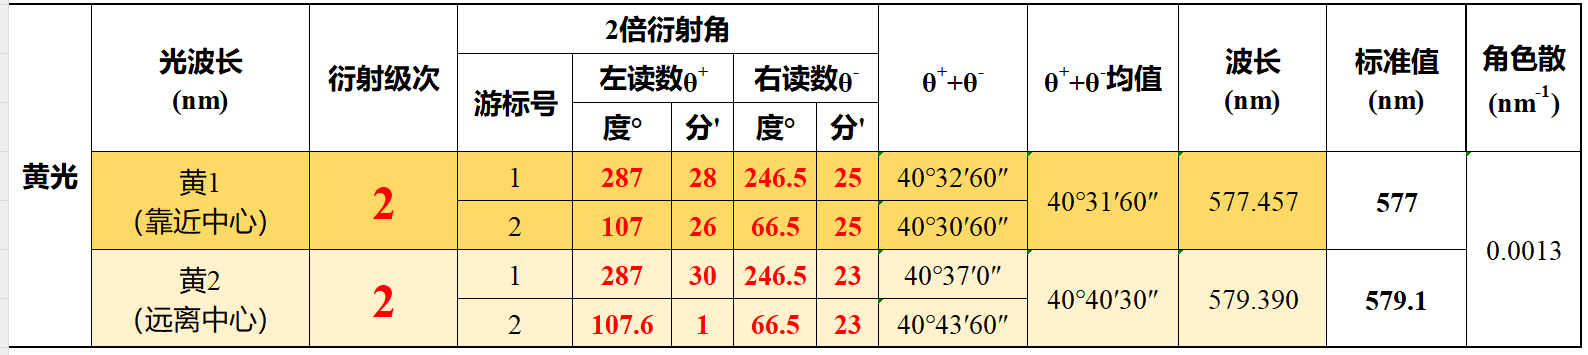
\includegraphics[width=12cm]{data2.png}
    \caption{测量汞黄双线波长实验数据}
\end{figure}\\
相对误差$E_1=\frac{\lambda_{1测量}-\lambda_{1理论}}{\lambda_{1理论}}\approx 7.92\times 10^{-4}$、$E_2=\frac{\lambda_{2测量}-\lambda_{2理论}}{\lambda_{2理论}}\approx 5.00\times 10^{-4}$
\section{思考题}
(1)\textbf{在调整好光路后,如果因为没有固定好物台,导致光栅所在物台旋转了
一个角度,即光线不是正入射光栅,会导致光栅衍射光谱发生什么变化?}\\
\hspace*{2em}斜入射时光栅方程变为
$$
d(\sin\theta_{i}+\sin\theta_{d})=k\lambda
$$
其中$\theta_{i}$为入射角,$\theta_{d}$为衍射角。这表明当物台旋转一个角度后,光栅衍射光谱会向一侧偏移。这使得某些原本可以观测到的光谱超出观测范围,有些原本观测不到的光谱则可能进入观测范围中。\\
\hspace*{2em}同时,由于光路发生改变,光走过的路程也发生改变,光谱的强度也会相应的发生改变。\\
(2)\textbf{描述衍射光谱颜色分布,分析其形成原因。}\\
\hspace*{2em}在光栅衍射形成的光谱中,颜色呈现出有规律的分布。一般来说,从中央零级条纹向两侧,会依次出现不同颜色的谱线。对于可见光波段,通常是按照紫、蓝、青、绿、黄、橙、红的顺序排列 。并且随着光谱级次k的增加,不同颜色谱线之间的间距会逐渐增大。\\
\hspace*{2em}原因:由光栅方程
$$
    d\sin \theta=k\lambda
$$
随着光谱级次$k$与波长$\lambda$的增加,$\theta$也相应的增加。\\
(3)\textbf{光栅衍射是一种多缝衍射,但其中也包含了单缝衍射,从该角度出发定性解释缺级现象的产生。}\\
\hspace*{2em}多缝衍射决定了衍射主极大的位置,单缝衍射决定了光强的分布,二者效果叠加从而产生了缺级现象。\\
(4)\textbf{如果实验中发现两条波长很近的谱线用该光栅无法分辨开,能否在光栅衍射后,通过放大光路将这两条谱线区分开?为什么?}\\
\hspace*{2em}根据光栅方程
$$
d\sin \theta=k\lambda
$$
放大光路无法改变光谱的角度差$\Delta\theta$,所以无法将两条谱线区分开来。\\
(5)\textbf{思考光栅衍射可以测量光波长、光栅常数外们还可能有什么应用?}\\
\hspace*{2em}光栅衍射还可以有以下应用:
\begin{itemize}
    \item 光谱分析:应用于天文学中对恒星、星系等天体的物质成分分析,以及化学、材料科学等领域对样品的元素组成进行定性和定量分析。
    \item 光通信:在密集波分复用(DWDM)技术中,光栅可作为波分复用器和解复用器。利用光栅对不同波长光的衍射角度不同,将多个不同波长的光信号复合到一根光纤中传输,在接收端再将各波长的光信号分离出来。
\end{itemize}
\section{总结}
\hspace*{2em}本次实验中,我们了解了分光仪和光栅的结构和原理,掌握了分光仪的调节(各半调节法)和使用,测定了光栅常数d和汞光谱中两条黄线的波长$\lambda$并计算了相应的角色散。
\end{document}